% Search for all the places that say "PUT SOMETHING HERE".

\documentclass[11pt]{article}
\usepackage{amsmath,textcomp,fancyvrb,pdfpages, amssymb,geometry,graphicx,enumerate,bm,hyperref}
\graphicspath{ {images/} }

\title{CS189--FALL 2015 --- Homework 7 Write up}
\author{ZUBO GU, SID 25500921, gu.zubo@berkeley.edu}
\markboth{}{}
\pagestyle{myheadings}
\date{}

\begin{document}
\maketitle

\section*{Problem 1}
\begin{itemize}
\item[1.2].
With K = 5, visualize the cluster centers as below.

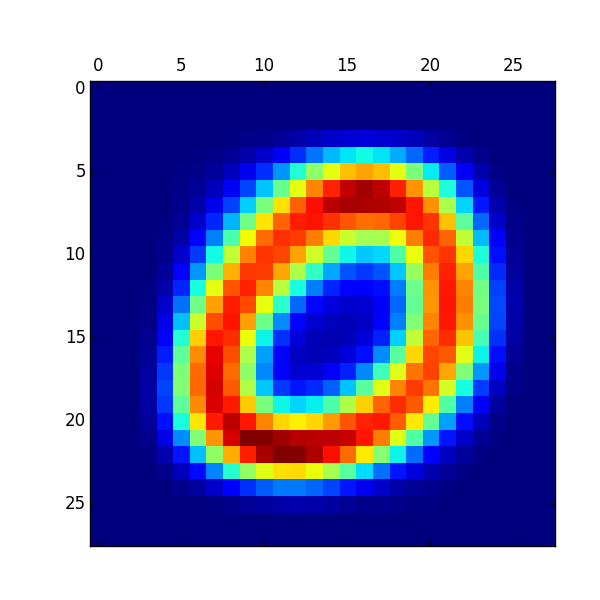
\includegraphics[scale = 0.5]{1.png}
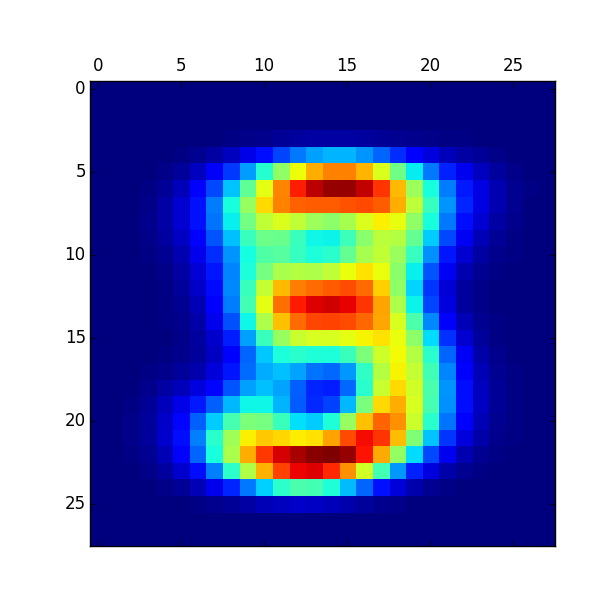
\includegraphics[scale = 0.5]{2.png}

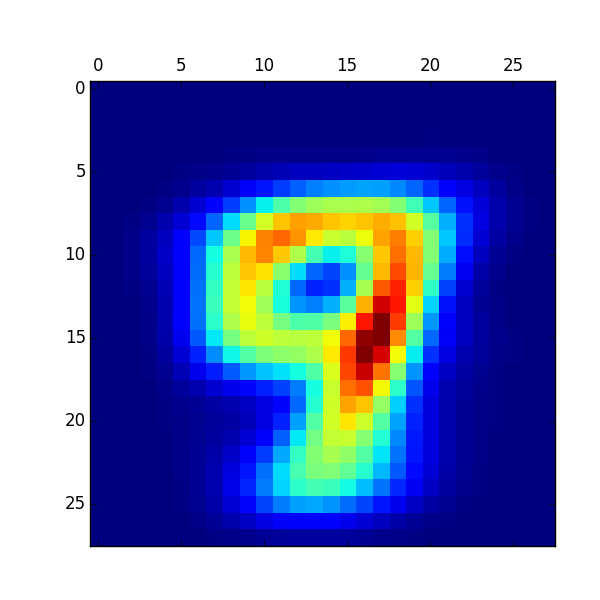
\includegraphics[scale = 0.5]{3.png}
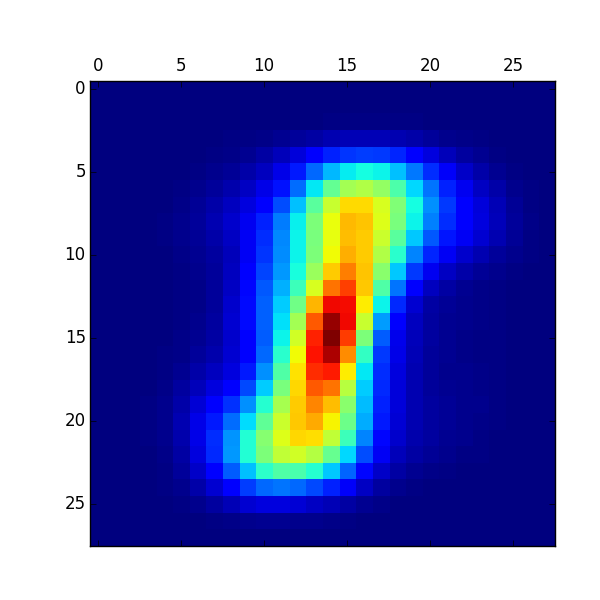
\includegraphics[scale = 0.5]{4.png}

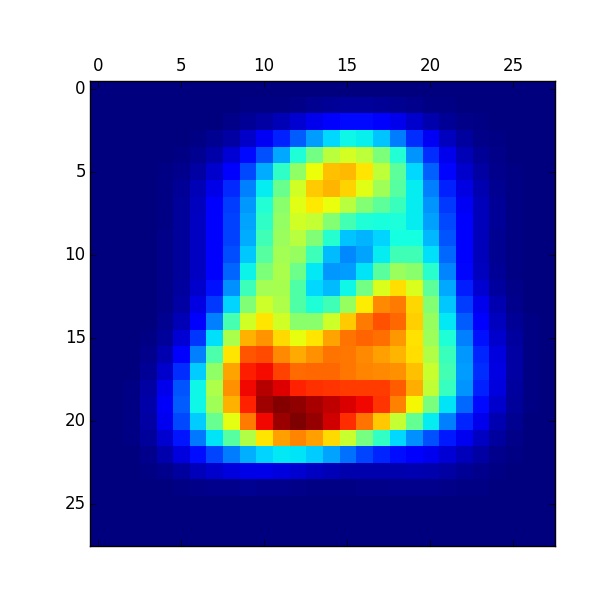
\includegraphics[scale = 0.5]{5.png}

With K = 10, visualize the cluster centers as below.

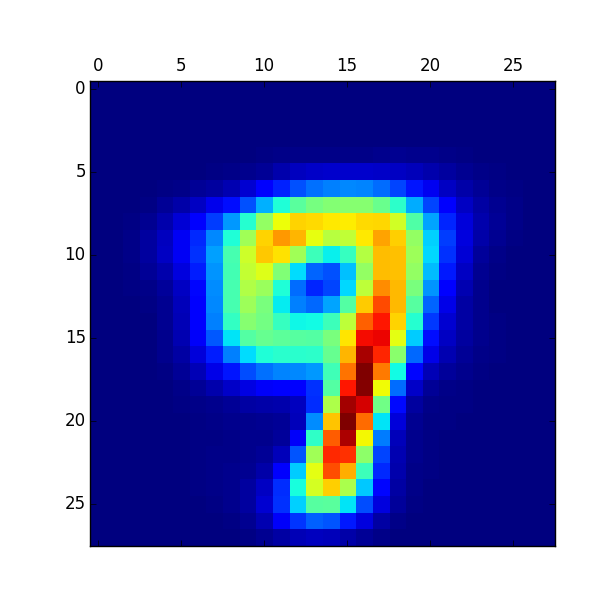
\includegraphics[scale = 0.5]{6.png}
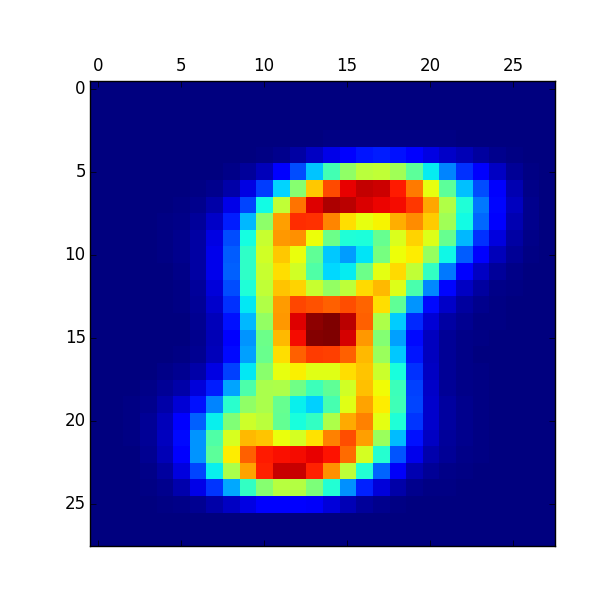
\includegraphics[scale = 0.5]{7.png}

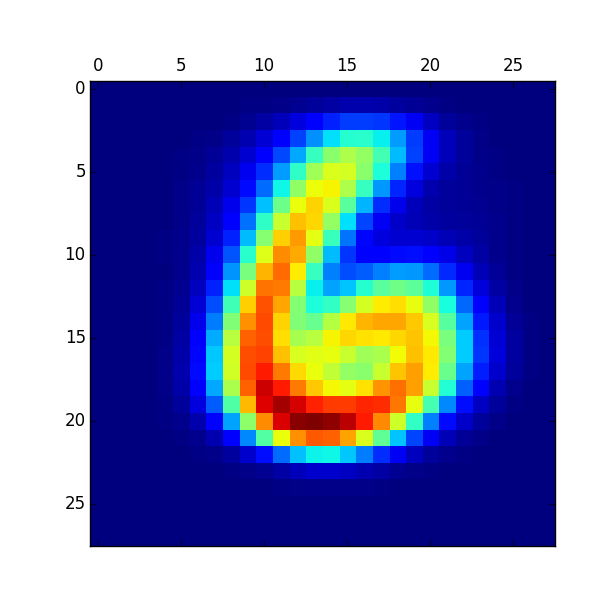
\includegraphics[scale = 0.5]{8.png}
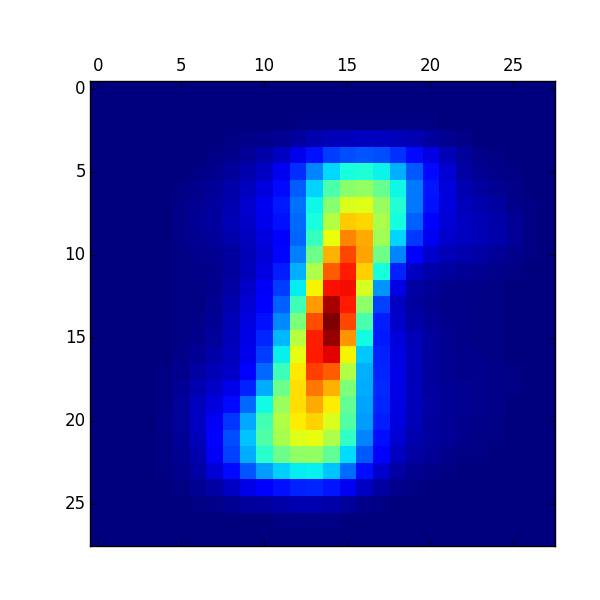
\includegraphics[scale = 0.5]{9.png}

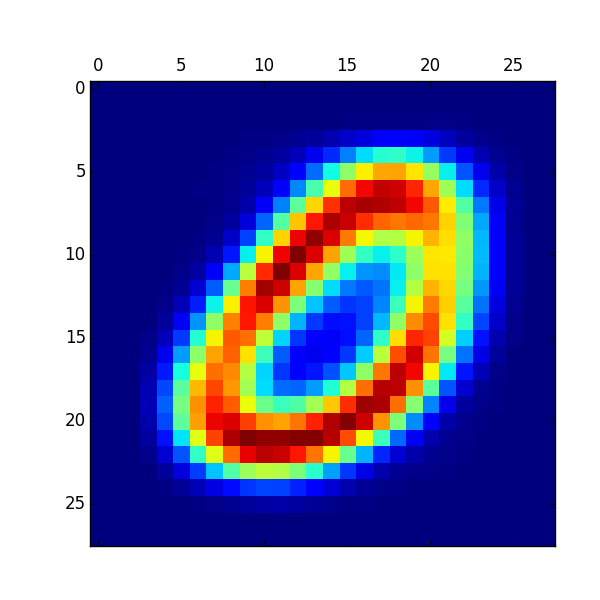
\includegraphics[scale = 0.5]{10.png}
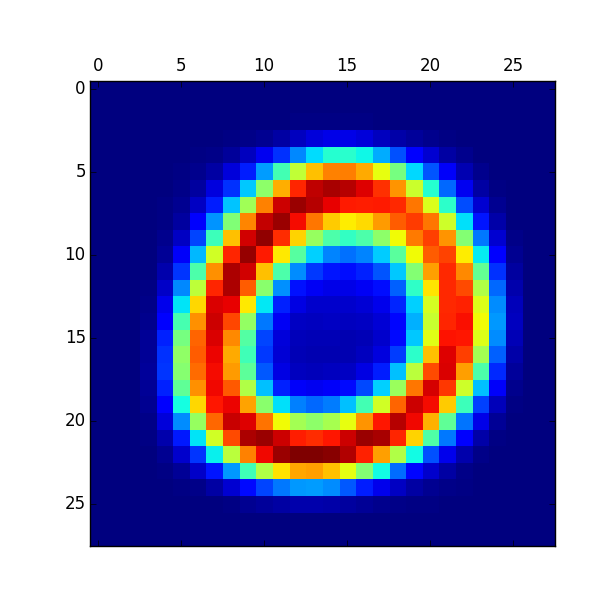
\includegraphics[scale = 0.5]{11.png}

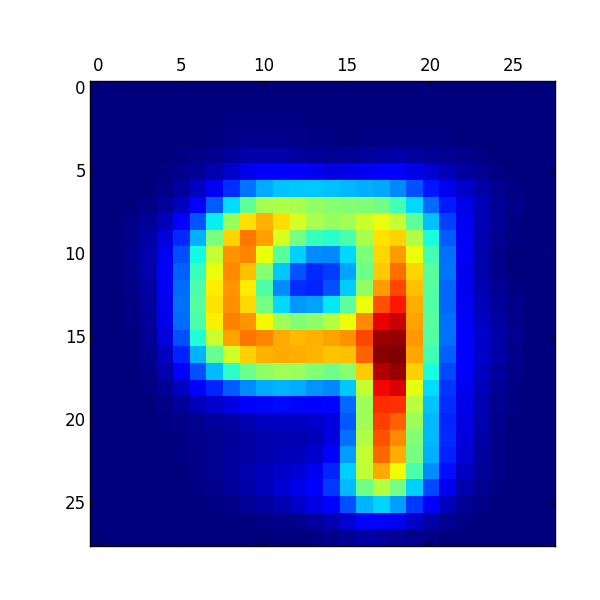
\includegraphics[scale = 0.5]{12.png}
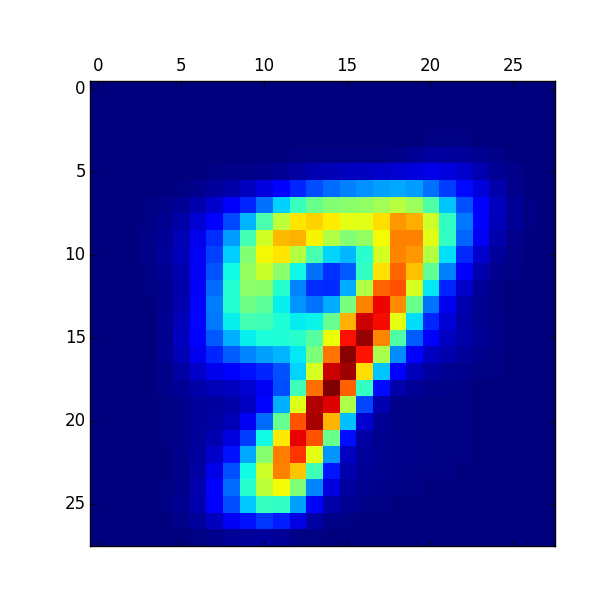
\includegraphics[scale = 0.5]{13.png}

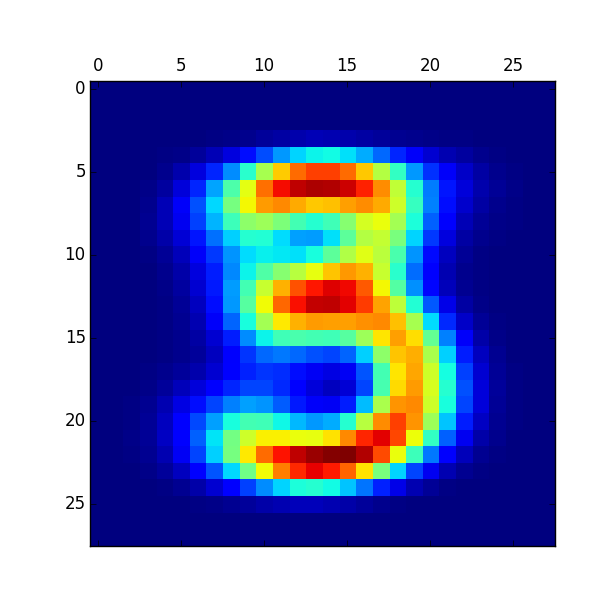
\includegraphics[scale = 0.5]{14.png}
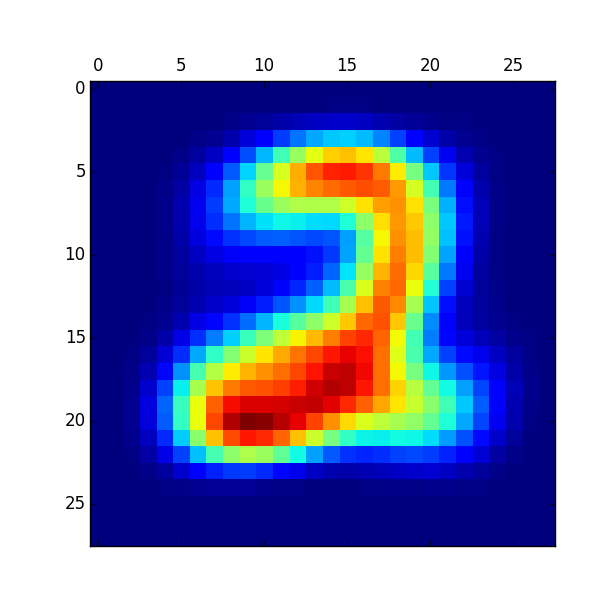
\includegraphics[scale = 0.5]{15.png}

With K = 20, visualize the cluster centers as below.

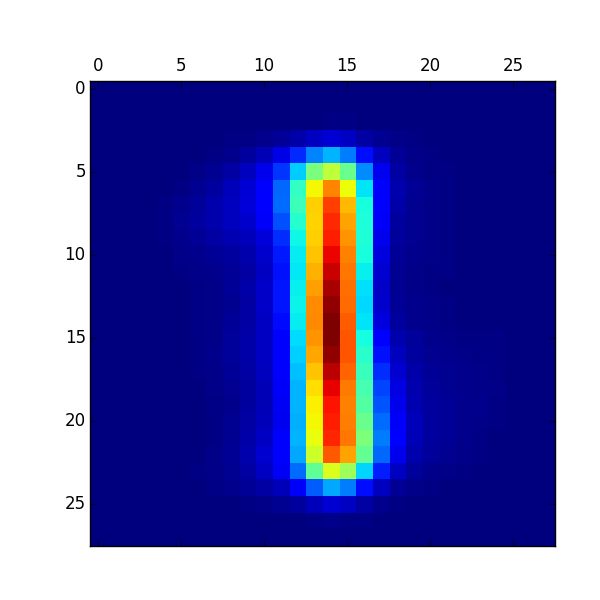
\includegraphics[scale = 0.5]{16.png}
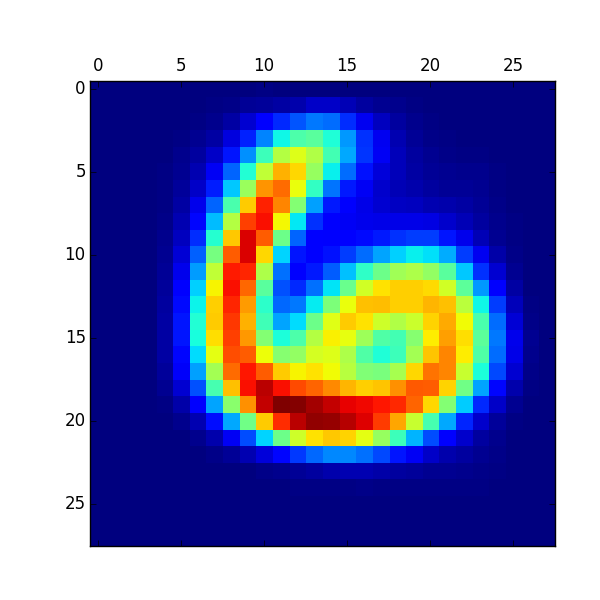
\includegraphics[scale = 0.5]{17.png}

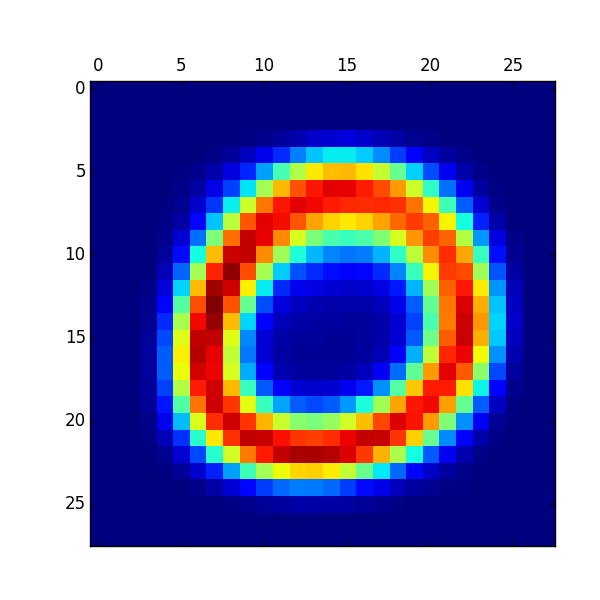
\includegraphics[scale = 0.5]{18.png}
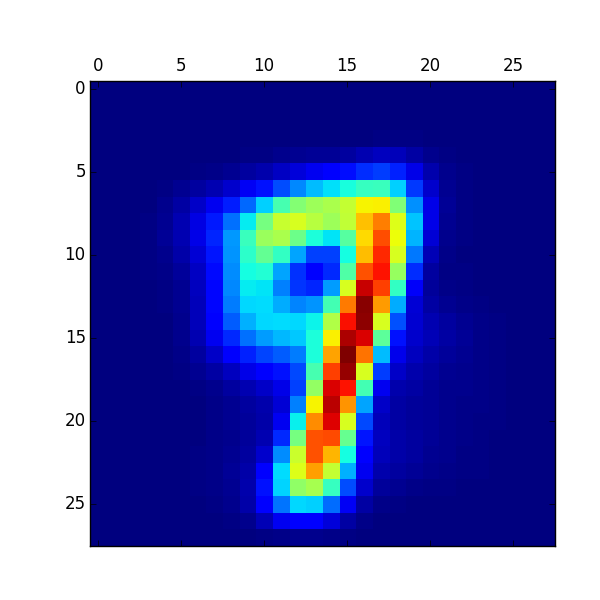
\includegraphics[scale = 0.5]{19.png}

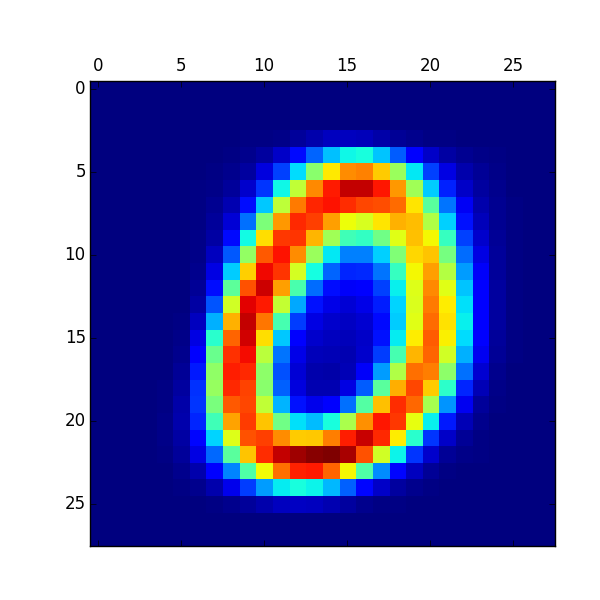
\includegraphics[scale = 0.5]{20.png}
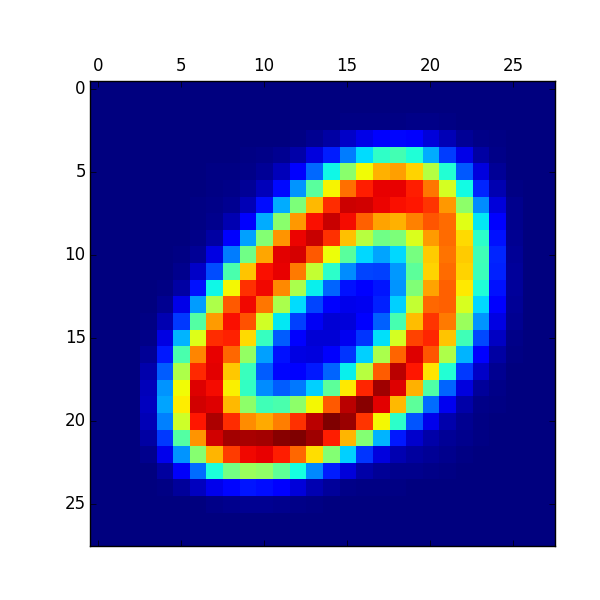
\includegraphics[scale = 0.5]{21.png}

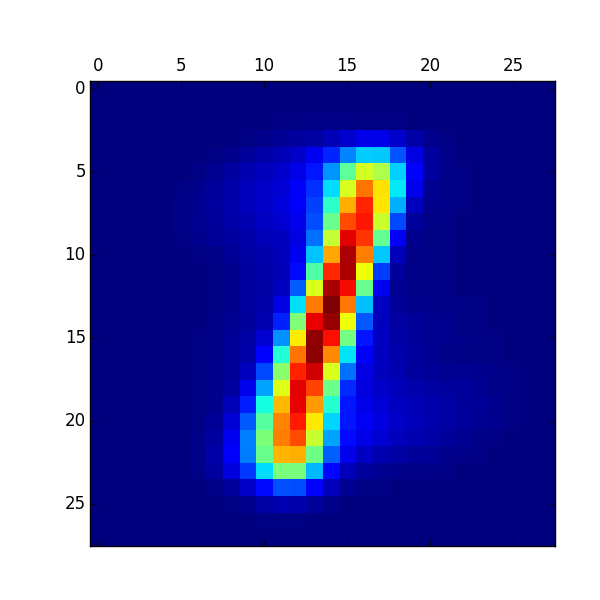
\includegraphics[scale = 0.5]{22.png}
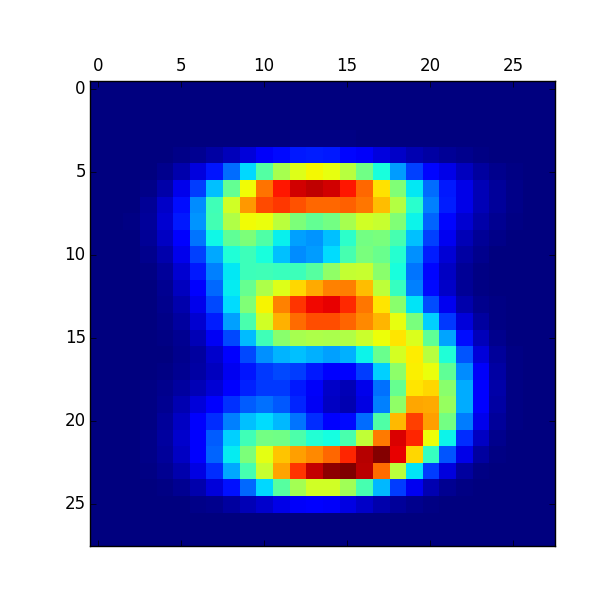
\includegraphics[scale = 0.5]{23.png}

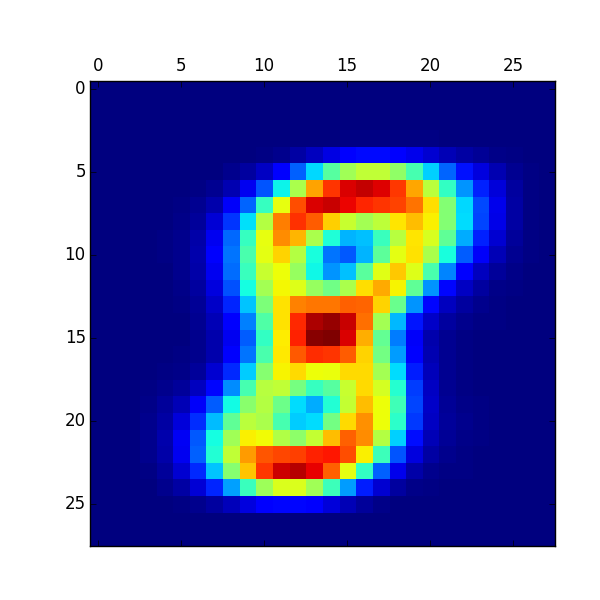
\includegraphics[scale = 0.5]{24.png}
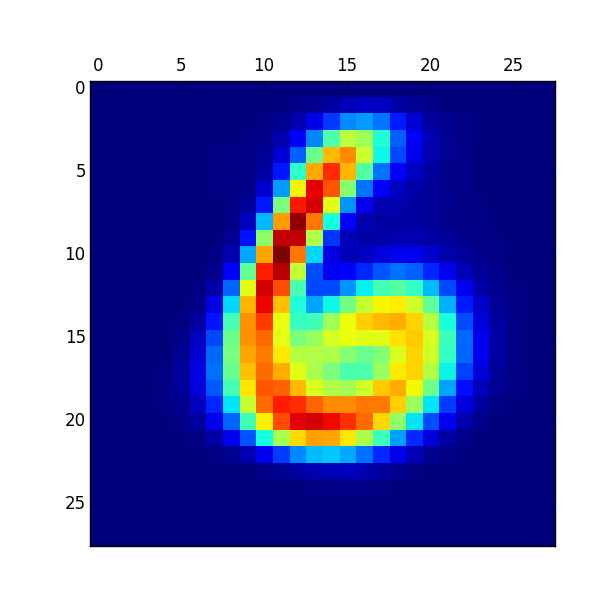
\includegraphics[scale = 0.5]{25.png}

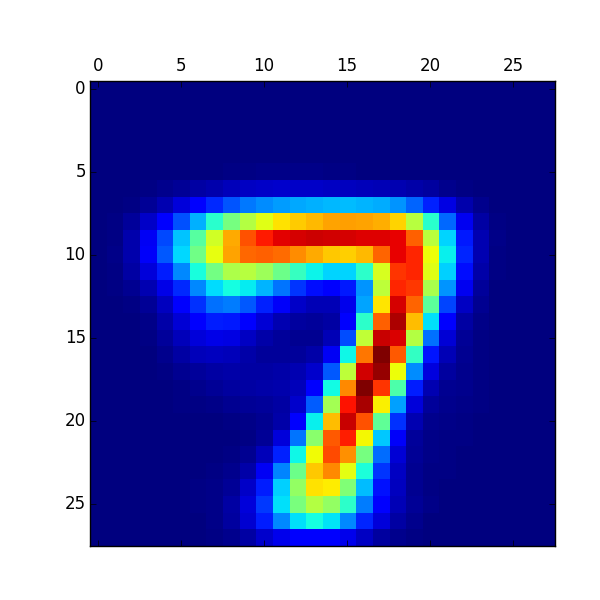
\includegraphics[scale = 0.5]{26.png}
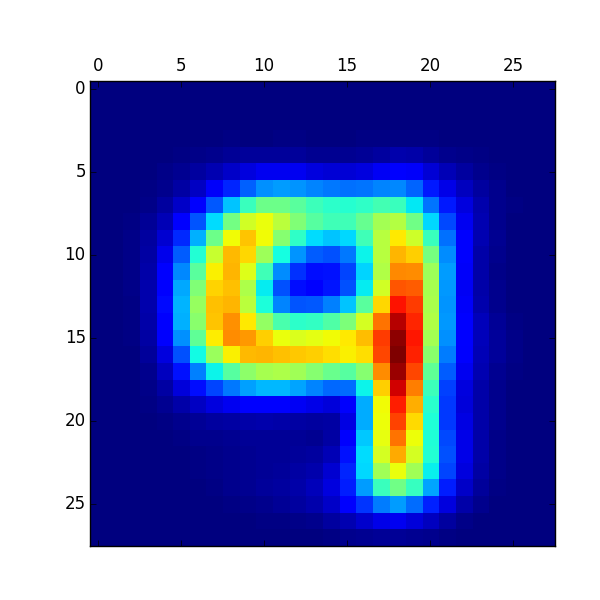
\includegraphics[scale = 0.5]{27.png}

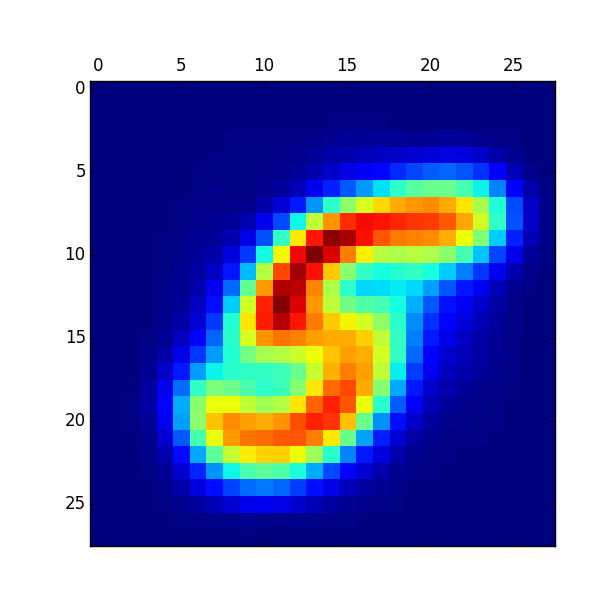
\includegraphics[scale = 0.5]{28.png}
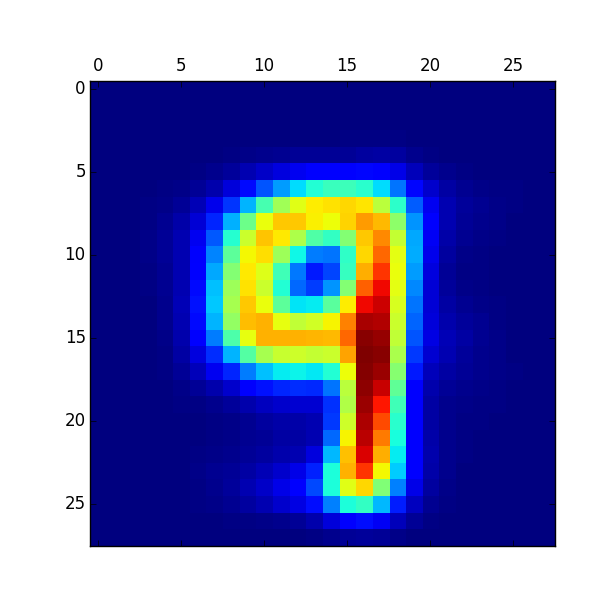
\includegraphics[scale = 0.5]{29.png}

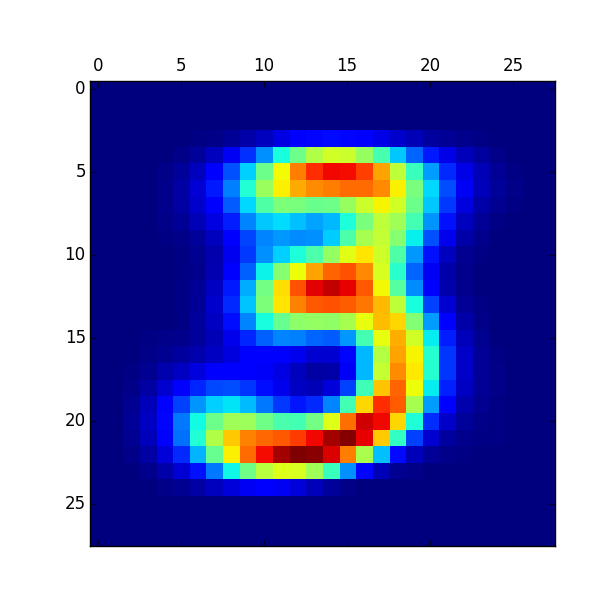
\includegraphics[scale = 0.5]{30.png}
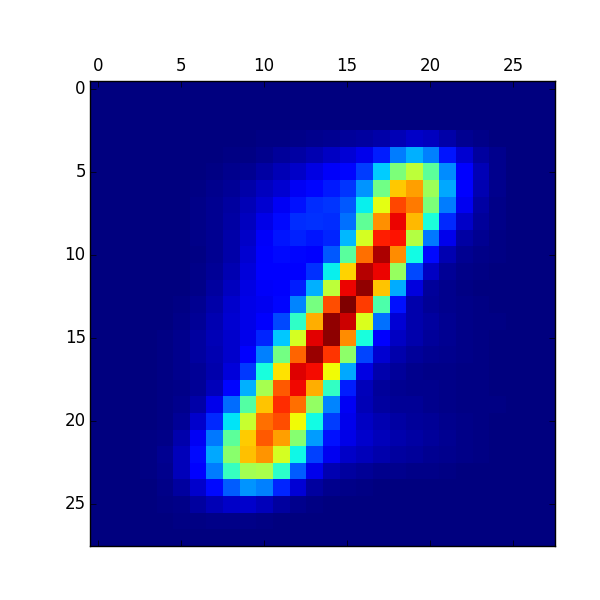
\includegraphics[scale = 0.5]{31.png}

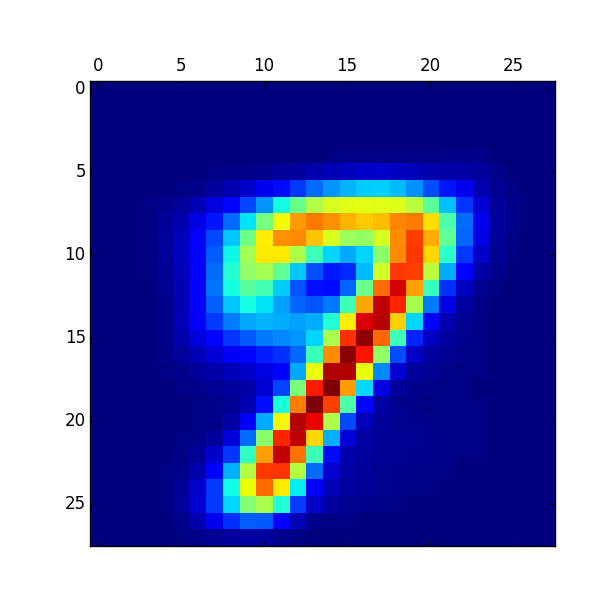
\includegraphics[scale = 0.5]{32.png}
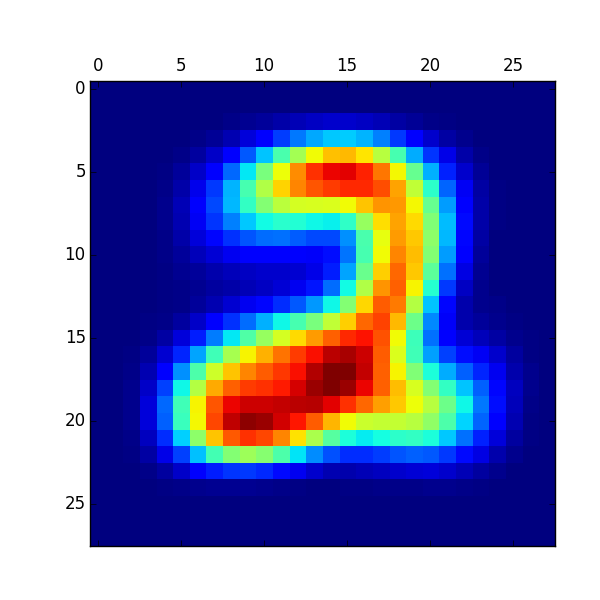
\includegraphics[scale = 0.5]{33.png}

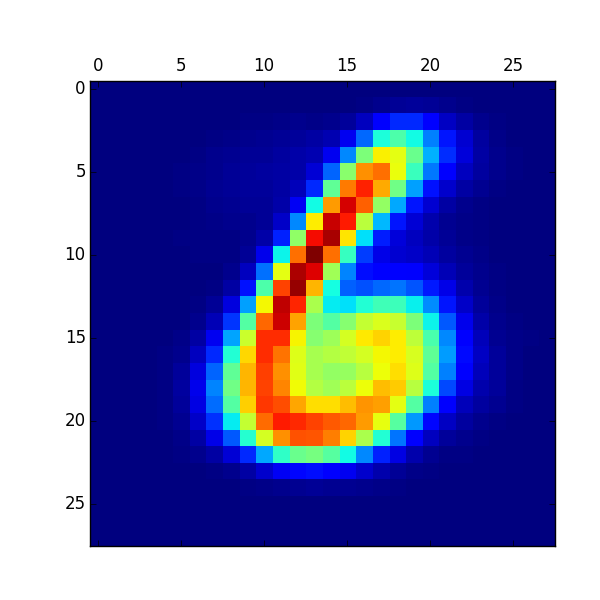
\includegraphics[scale = 0.5]{34.png}
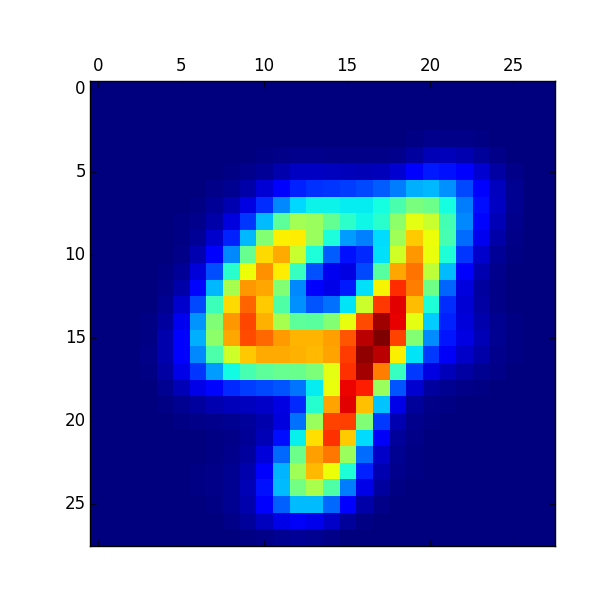
\includegraphics[scale = 0.5]{35.png}

\item[1.3].

the k-mean loss does vary in different runs.

\end{itemize}

\section*{Problem 2}
\begin{itemize}
\item[2.2].

Recommend the joke by its average rating in the training set, the validation set accuracy is 0.6203252032520326

Find the k nearest neighbors of him/her, then make the prediction by averaging the ratings of these neighbors.

With K = 10, the validation set accuracy is 0.6490514905149052

With K = 100, the validation set accuracy is 0.6894308943089431

With K = 1000, the validation set accuracy is  0.6940379403794038

The accuracies are all higher than the accuracy that we got from the simple system.

\item[2.3.1].
See code in q2.3.py

\item[2.3.2].

MSE is 20257100.7948 for d =  2

Validation Set accuracy is  0.7094850948509485 for d =  2

MSE is 18839053.5157 for d =  5

Validation Set accuracy is  0.713550135501355 for d =  5

MSE is 17092099.6887 for d =  10

Validation Set accuracy is  0.7132791327913279 for d =  10

MSE is 14192908.8435 for d =  20

Validation Set accuracy is  0.6859078590785908 for d =  20

Thus, MSE is decrease as variable d increase.

\item[2.3.3].
See code in q2.3.3.py

\item[2.3.4].

MSE is 15111947.0226 for d =  2

Validation Set accuracy is  0.7073170731707317 for d =  2

MSE is 12380230.026 for d =  5

Validation Set accuracy is  0.7092140921409215 for d =  5

MSE is 9632977.97809 for d =  10

Validation Set accuracy is  0.7184281842818429 for d =  10

MSE is 5656292.52527 for d =  20

Validation Set accuracy is  0.6658536585365854 for d =  20


Compare to step 2, for the same d value, the MSE in is much lower in step 3. The validation set accuracies are almost same in both step 2 and 3, not having significant difference. 

\item[2.4].

The best kaggle result is 0.72573

\end{itemize}

\newpage
\section*{Code Q1}
\VerbatimInput[baselinestretch=1,fontsize=\footnotesize,numbers=left]{q1.py}

\newpage
\section*{Code Q2.2}
\VerbatimInput[baselinestretch=1,fontsize=\footnotesize,numbers=left]{q2_2.py}

\newpage
\section*{Code Q2.3.2}
\VerbatimInput[baselinestretch=1,fontsize=\footnotesize,numbers=left]{q2_3_2.py}

\newpage
\section*{Code Q2.3.3}
\VerbatimInput[baselinestretch=1,fontsize=\footnotesize,numbers=left]{q2_3_3.py}

\end{document}


